\documentclass[10pt,twocolumn]{article}
\usepackage[margin=0.72in]{geometry}
\usepackage{graphicx}
\usepackage{booktabs}
\usepackage{amsmath,amssymb}
\usepackage{microtype}
\usepackage{enumitem}
\usepackage{xcolor}
\usepackage{url}
\usepackage[hidelinks]{hyperref}
\setlength{\columnsep}{0.23in}
\setlist{nosep,leftmargin=*}
\hyphenpenalty=5000
\exhyphenpenalty=5000
\emergencystretch=1em

\title{\textbf{Layerwise Behavioral Sensitivity in LLMs: Stability, Scale, and the Limits of Capability Localization}}
\author{Srinivas Velpuri\\Andyur AI\\\href{mailto:svelpuri@andyur.ai}{svelpuri@andyur.ai}\\ORCID: \href{https://orcid.org/0009-0005-8111-2622}{0009-0005-8111-2622}}
\date{}

\begin{document}
\maketitle

\begin{abstract}
A common approach to localizing capabilities in large language models is to intervene on internal components and measure behavioral degradation. Yet high intervention sensitivity may reflect general model disruption rather than selective involvement in the measured behavior. We study this question using preserved whole-block intervention measurements from Qwen3-0.6B and Qwen3-1.7B as an empirical testbed. Every transformer block was individually bypassed and evaluated on tool selection, argument binding, full-call correctness, and collateral perplexity. We first measure the reproducibility of layer sensitivity rankings within observed samples, then model tool-task damage as a function of relative perplexity degradation and analyze residual tool sensitivity beyond this general-damage proxy. Split-half tool-selection rankings are highly reproducible within discovery samples (median Spearman $\rho=0.931$ for 0.6B and $0.876$ for 1.7B). Perplexity degradation explains only a modest fraction of tool-task damage ($R^2\approx0.08$ for 0.6B and $0.28$ for 1.7B). Conservative robustness checks identify eight excess-sensitive blocks in 0.6B and three in 1.7B; the sets do not overlap. Cross-size residual-profile correlations are weak ($\rho\approx0.27$--$0.29$). These results support reproducible, intervention-specific behavioral sensitivity, but not unique or stable capability locations. The evidence is deliberately narrow: the primary endpoint contains 20 discovery tool examples, the general-damage proxy uses five perplexity documents, both models are from one family, and Phase 5 has no held-out per-layer intervention map. A richer collateral-behavior panel could change which blocks appear excess-sensitive. We therefore argue for a strict distinction between general component importance, behavioral sensitivity, and capability localization.
\end{abstract}

\section{Introduction}
Large language models exhibit apparently distinct behaviors such as tool use, arithmetic, factual retrieval, structured output, and planning. If these behaviors depend selectively on identifiable internal components, localization could guide model editing, compression, safety interventions, and parameter-efficient adaptation. Prior work has reported task-related layer transitions \cite{zhao2024layer}, functionally selective units \cite{alkhamissi2025llm}, skill neurons \cite{wang2022skill}, and knowledge-associated neurons or MLP computations \cite{dai2022knowledge,meng2022rome}.

However, three concepts are often conflated: a component can \emph{represent} information, be \emph{causally important} under a particular intervention, or be a good \emph{place to modify} behavior. These need not coincide. Causal localization of factual knowledge does not reliably identify the best editing location \cite{hase2023localization}; activation-patching conclusions can depend strongly on methodological choices \cite{zhang2024patching}; and recent work finds factual computation to be redundant, distributed, and non-contiguous \cite{hochman2026factual}.

We therefore ask a narrower question: \textbf{when bypassing a layer causes large tool-task damage, how much of that damage exceeds the general disruption measured by the same intervention?}

The study reanalyzes preserved measurements from a broader Capability Anatomy project. It is intentionally not a claim that a ``tool-use layer'' has been found. Instead, it evaluates how far intervention evidence can support localization language.

\paragraph{Contributions.} Using Qwen3-0.6B and Qwen3-1.7B as a controlled empirical testbed, we provide four contributions:
\begin{enumerate}
  \item a reproducibility analysis of whole-block tool-calling sensitivity in two Qwen3 sizes;
  \item a conditional specificity analysis that separates tool-task damage from a retained perplexity-damage proxy;
  \item robustness criteria that avoid treating catastrophic general-damage blocks as capability-specific sites; and
  \item an explicit claim boundary distinguishing reproducible intervention effects from capability localization.
\end{enumerate}

\begin{figure*}[t]
\centering
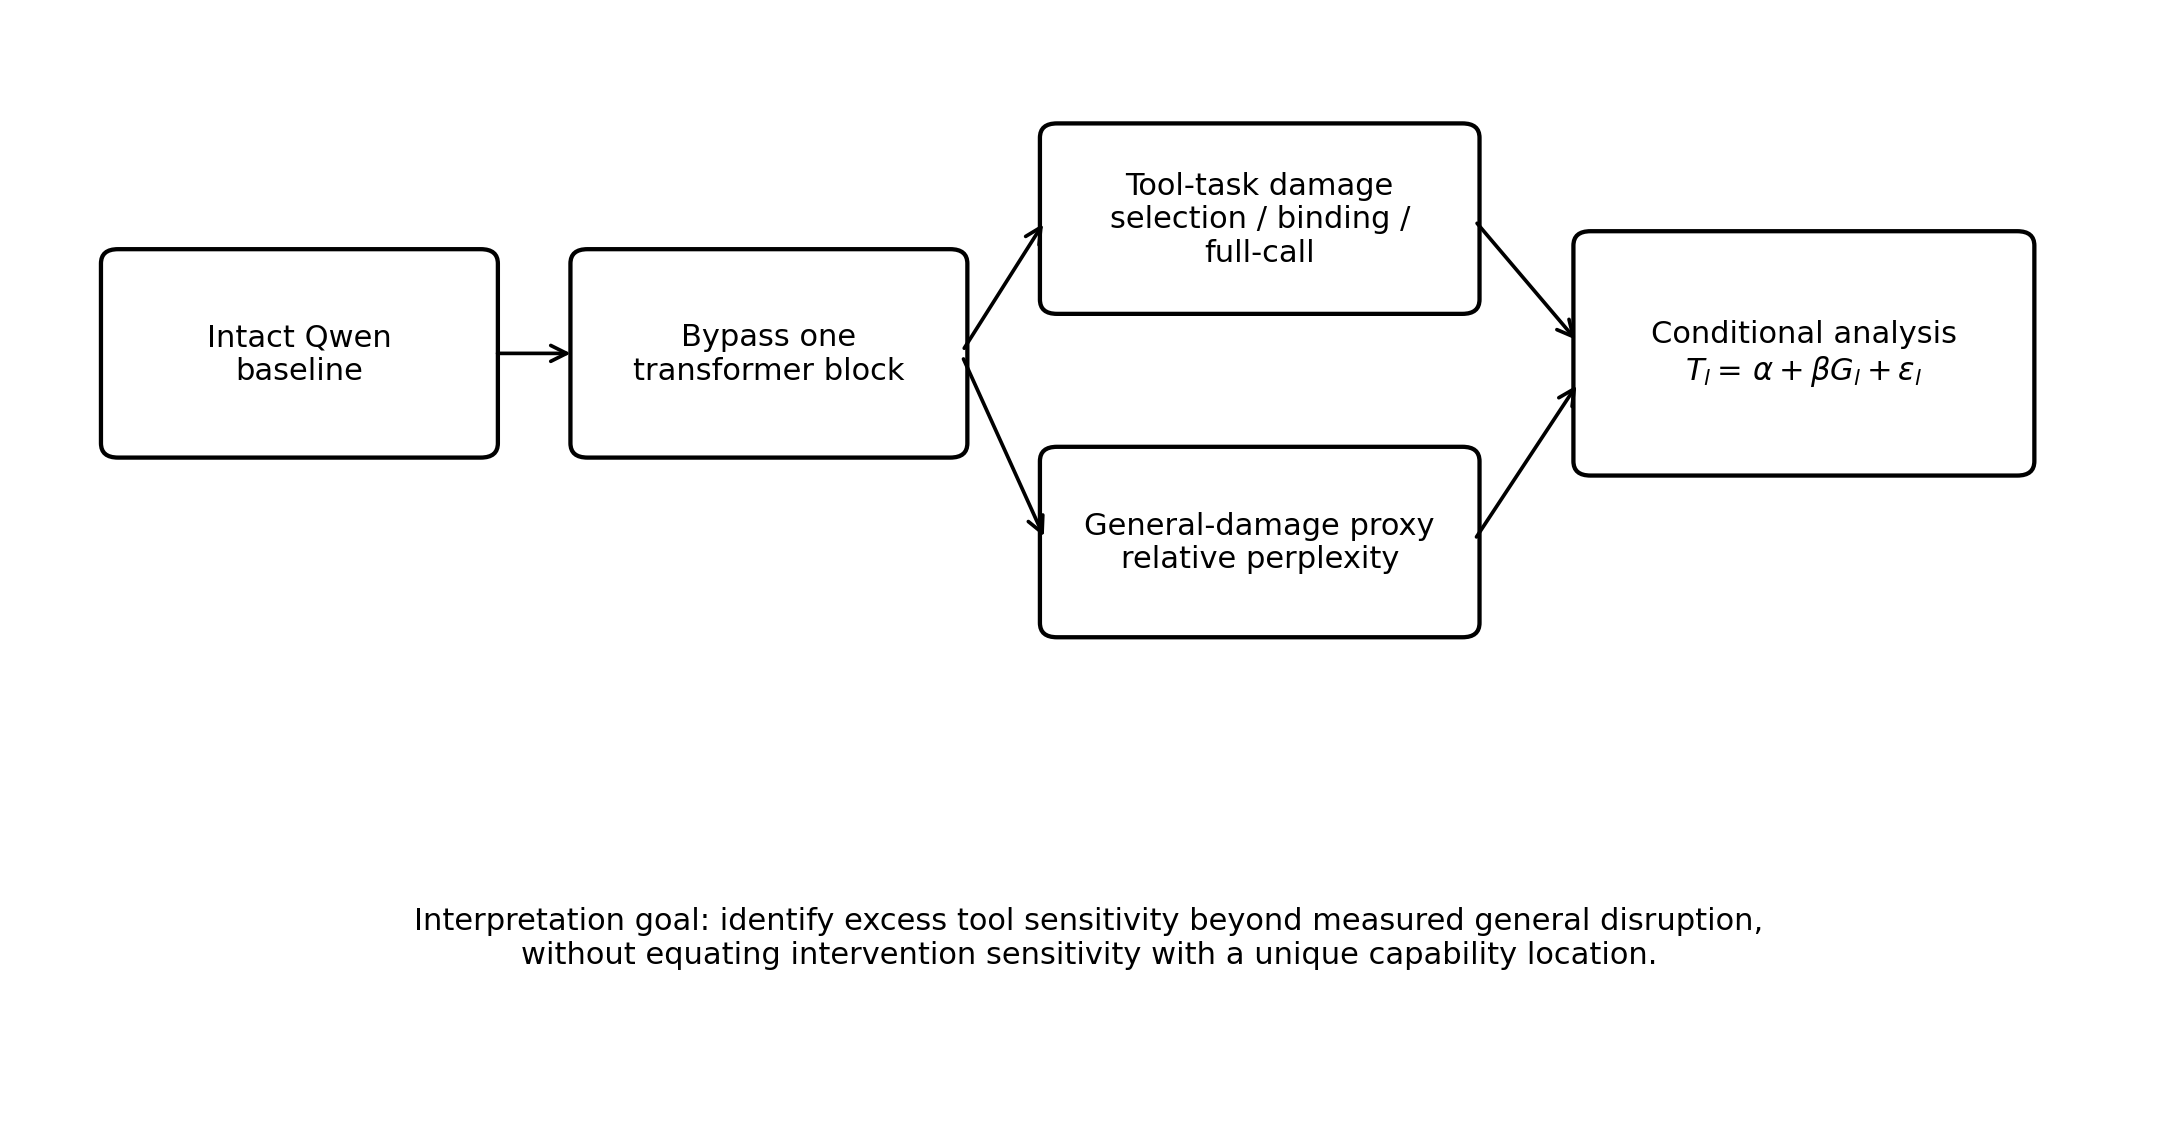
\includegraphics[width=0.94\textwidth]{figure1_workflow.png}
\caption{Analysis workflow. Whole-block bypass yields target tool-task damage and collateral perplexity damage. The residual analysis asks whether tool degradation exceeds that predicted by the measured general-damage proxy.}
\label{fig:workflow}
\end{figure*}

\section{Related Work}
\paragraph{Functional and task localization.}
Layerwise representation analyses report transitions from shared to task-oriented representations \cite{zhao2024layer}. Functional localization has identified causally task-relevant units across many LLMs, including language-selective subnetworks and specialization in some reasoning and social tasks \cite{alkhamissi2025llm}. Earlier neuron-level studies identified task-associated skill neurons \cite{wang2022skill} and fact-associated knowledge neurons \cite{dai2022knowledge}.

\paragraph{Localization, editing, and methodological dependence.}
ROME linked factual recall to mid-layer feed-forward computations and used these observations to motivate editing \cite{meng2022rome}. Later work showed that causal-tracing localization does not reliably predict which layer is best to edit \cite{hase2023localization}. More recent editing work identifies a robustness--specificity tension in the semantic keys used by locate-and-edit methods \cite{yan2025robust}, while localization-informed deletion of toxic memories can outperform random early-layer editing under a toxicity--perplexity trade-off \cite{das2025toxic}. Together, these results suggest that localization can sometimes be operationally useful without making it a universal or method-independent property. Activation-patching studies likewise show that metrics and corruption choices can materially change localization conclusions \cite{zhang2024patching}.

\paragraph{Distributed computation and layer removal.}
Recent evidence suggests that factual retrieval can depend on multiple non-contiguous, functionally equivalent pathways \cite{hochman2026factual}. Separately, TrimLLM exploits layer-wise specialization to drop layers for domain-specific models, showing that some layer removal can be useful under domain specialization \cite{hu2025trimllm}. Our work differs by focusing on tool-calling sensitivity, controlling descriptively for general perplexity damage, and emphasizing limits on localization claims.

\section{Evidence and Experimental Setup}
\subsection{Models and retained runs}
We analyze preserved Phase 5 measurements for Qwen3-0.6B and Qwen3-1.7B. Both intervention topologies expose 28 transformer blocks. Each run contains 3,400 observations: 33 discovery conditions over 50 items with two deterministic repetitions, plus a validation baseline. Discovery conditions include 28 individual block bypasses, intact baselines, a no-op, and one duplicate-block reproducibility control. The validation plan contains no per-layer intervention map; therefore held-out localization stability is not claimed.

The complete 1.7B evidence bundle contains 101 files and was preserved as an immutable byte-verified archive before the present analysis. The paper analysis uses only stored observations and performs no model loading or inference.

\subsection{Target and collateral measurements}
The primary target metrics are tool selection, argument binding, and full-call correctness. Tool selection is the clearest endpoint. Binding and full-call are nearly collinear in the retained data and are treated as related outcomes rather than independent confirmations.

Historical abstention, reasoning, and format metrics are excluded from the primary specificity claims because the evidence audit identified scorer and floor/duplication limitations.

For a block $l$, target damage is
\begin{equation}
T_l=\bar{s}_{\mathrm{intact}}-\bar{s}_l.
\end{equation}
Relative perplexity damage is
\begin{equation}
G_l=\frac{\overline{\mathrm{PPL}}_l}{\overline{\mathrm{PPL}}_{\mathrm{intact}}}-1.
\end{equation}
Perplexity is measured on five retained documents per model. It is a limited general-damage proxy, not a measurement of preservation of all unrelated capabilities.

\begin{figure}[t]
\centering
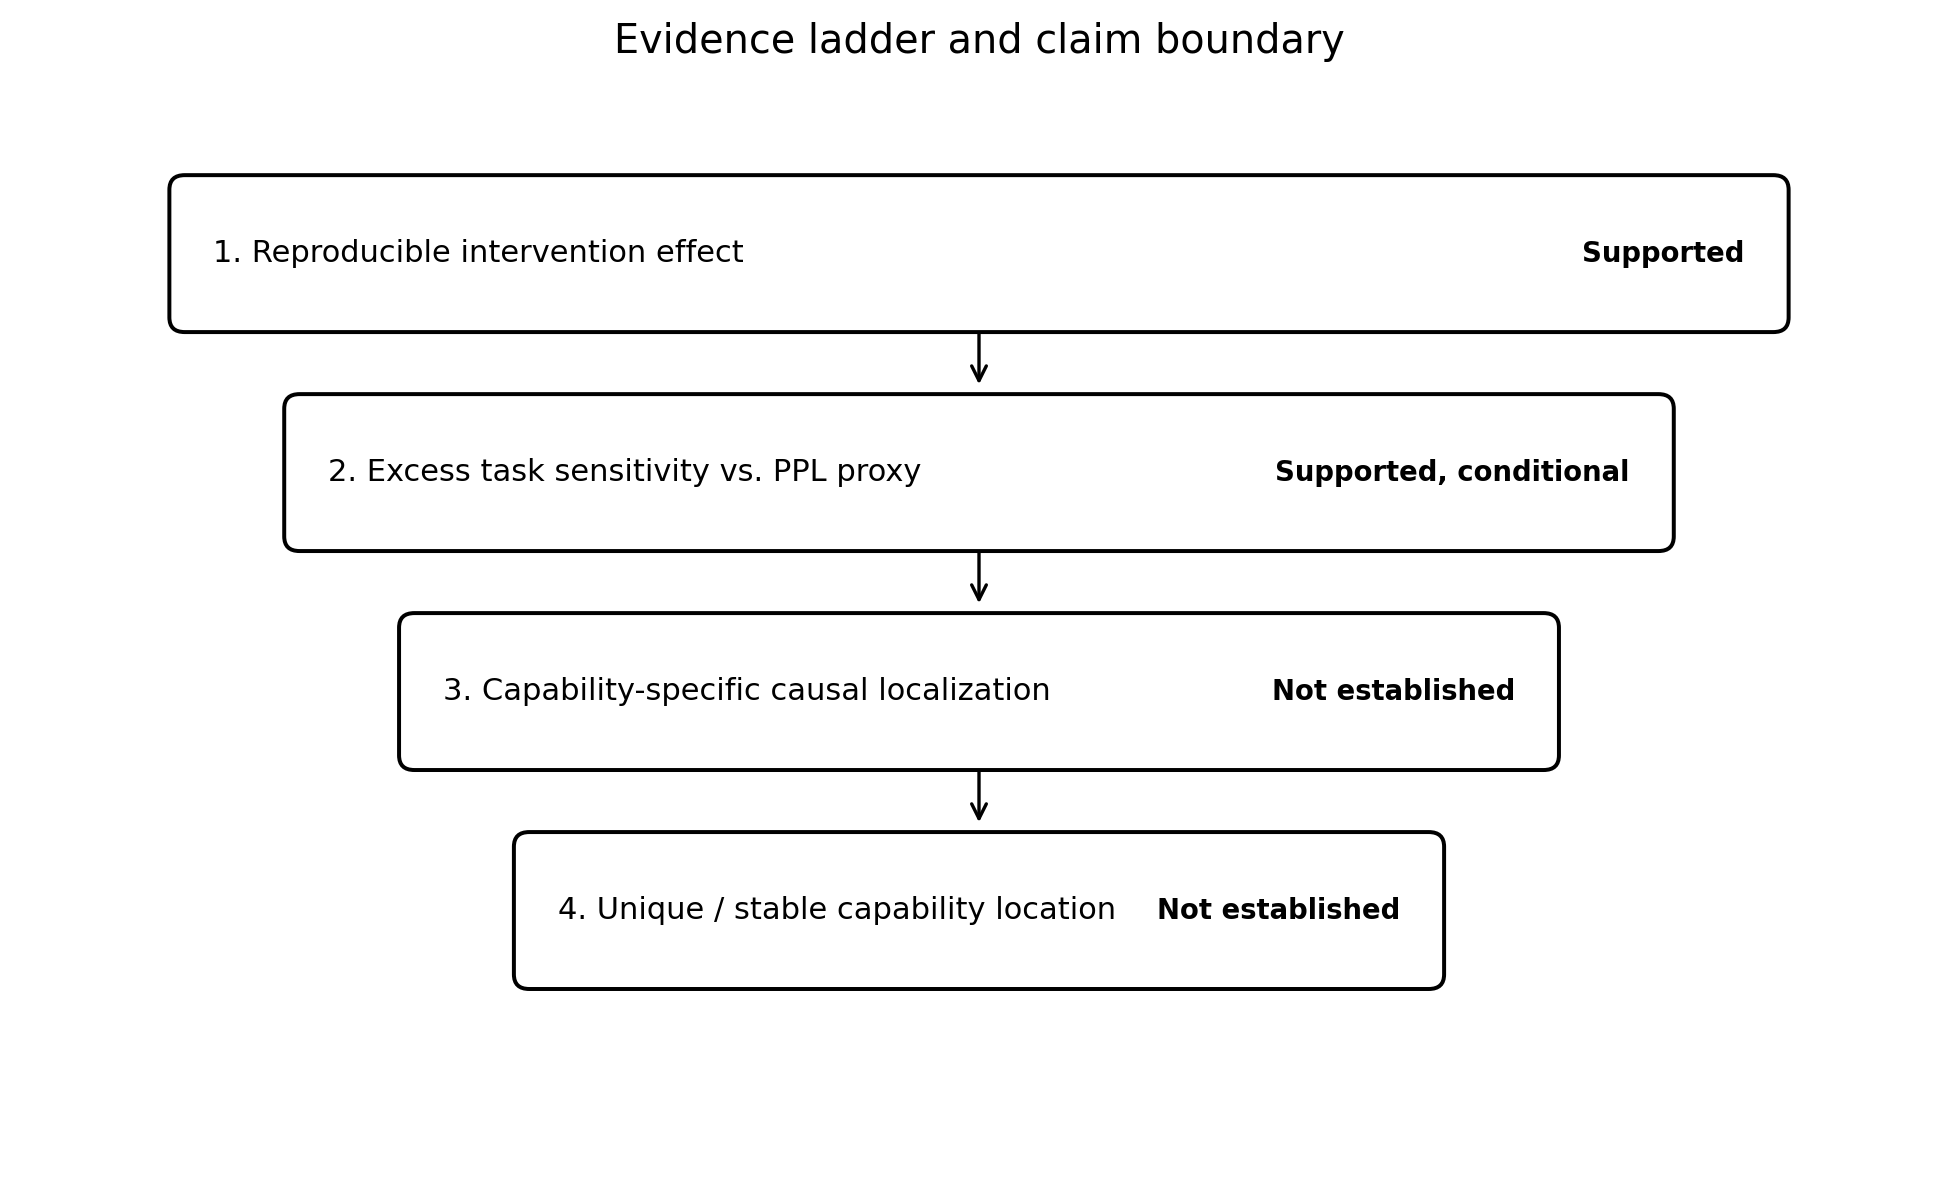
\includegraphics[width=\columnwidth]{figure2_claim_boundary.png}
\caption{Claim boundary. Each stronger interpretation requires evidence not supplied by the preceding level.}
\label{fig:claim}
\end{figure}

\subsection{Conditional specificity analysis}
For each target metric we fit
\begin{equation}
T_l=\alpha+\beta\log(1+G_l)+\epsilon_l.
\end{equation}
The residual $\epsilon_l$ describes tool-task damage not captured by this fitted perplexity relation. Raw-relative $G_l$ is retained as a robustness specification. We also use leave-one-layer-out prediction and monotone isotonic regression to assess shape sensitivity.

A residual of 0.10 (10 percentage points) is used as a descriptive materiality threshold. This was fixed in the post-hoc analysis plan before fitting, but is not a historical preregistered criterion.

\subsection{Uncertainty and independence}
The independent resampling units are 20 distinct tool examples and five perplexity documents per model. Deterministic repetitions are collapsed. We use 10,000 paired bootstrap draws and preserve the full vector of layer responses in each draw. Approximate simultaneous 95\% bands are formed across 336 residuals (two sizes $\times$ three targets $\times$ 28 layers $\times$ two regression specifications). Layers are not treated as 28 independent sampled experimental units; layerwise $t$-tests are not used.

\section{Results}
\subsection{Within-sample reproducibility}
Random 10/10 splits of the 20 discovery tool examples yield median split-half tool-selection rank correlations of $0.931$ for Qwen3-0.6B and $0.876$ for Qwen3-1.7B. The central 95\% resampling ranges are 0.863--0.958 and 0.808--0.923. These values show substantial reliability within the observed discovery sample; they are not independent held-out validation.

An older aggregate Phase 0B experiment does contain discovery and validation damage matrices. Tool-selection rank correlations are 0.865 for Qwen3-1.7B and 0.396 for Qwen3-4B. Because those matrices are aggregate-only, small, and use a different protocol, they are supporting evidence rather than pooled estimates.

\subsection{Perplexity is an incomplete explanation of target damage}
Table~\ref{tab:r2} summarizes the primary log-relative PPL regressions. Perplexity explains about 8\% of target-damage variance in 0.6B and 28\% in 1.7B. This establishes only that the chosen proxy/fit is incomplete; it does not identify the unmeasured cause.

\begin{table}[t]
\centering
\caption{Coefficient of determination ($R^2$) for tool-task damage regressed on log-relative perplexity damage.}
\label{tab:r2}
\begin{tabular}{lccc}
\toprule
Model & Selection & Binding & Full call \\
\midrule
Qwen3-0.6B & .0839 & .0831 & .0828 \\
Qwen3-1.7B & .2789 & .2761 & .2761 \\
\bottomrule
\end{tabular}
\end{table}

\begin{figure}[t]
\centering
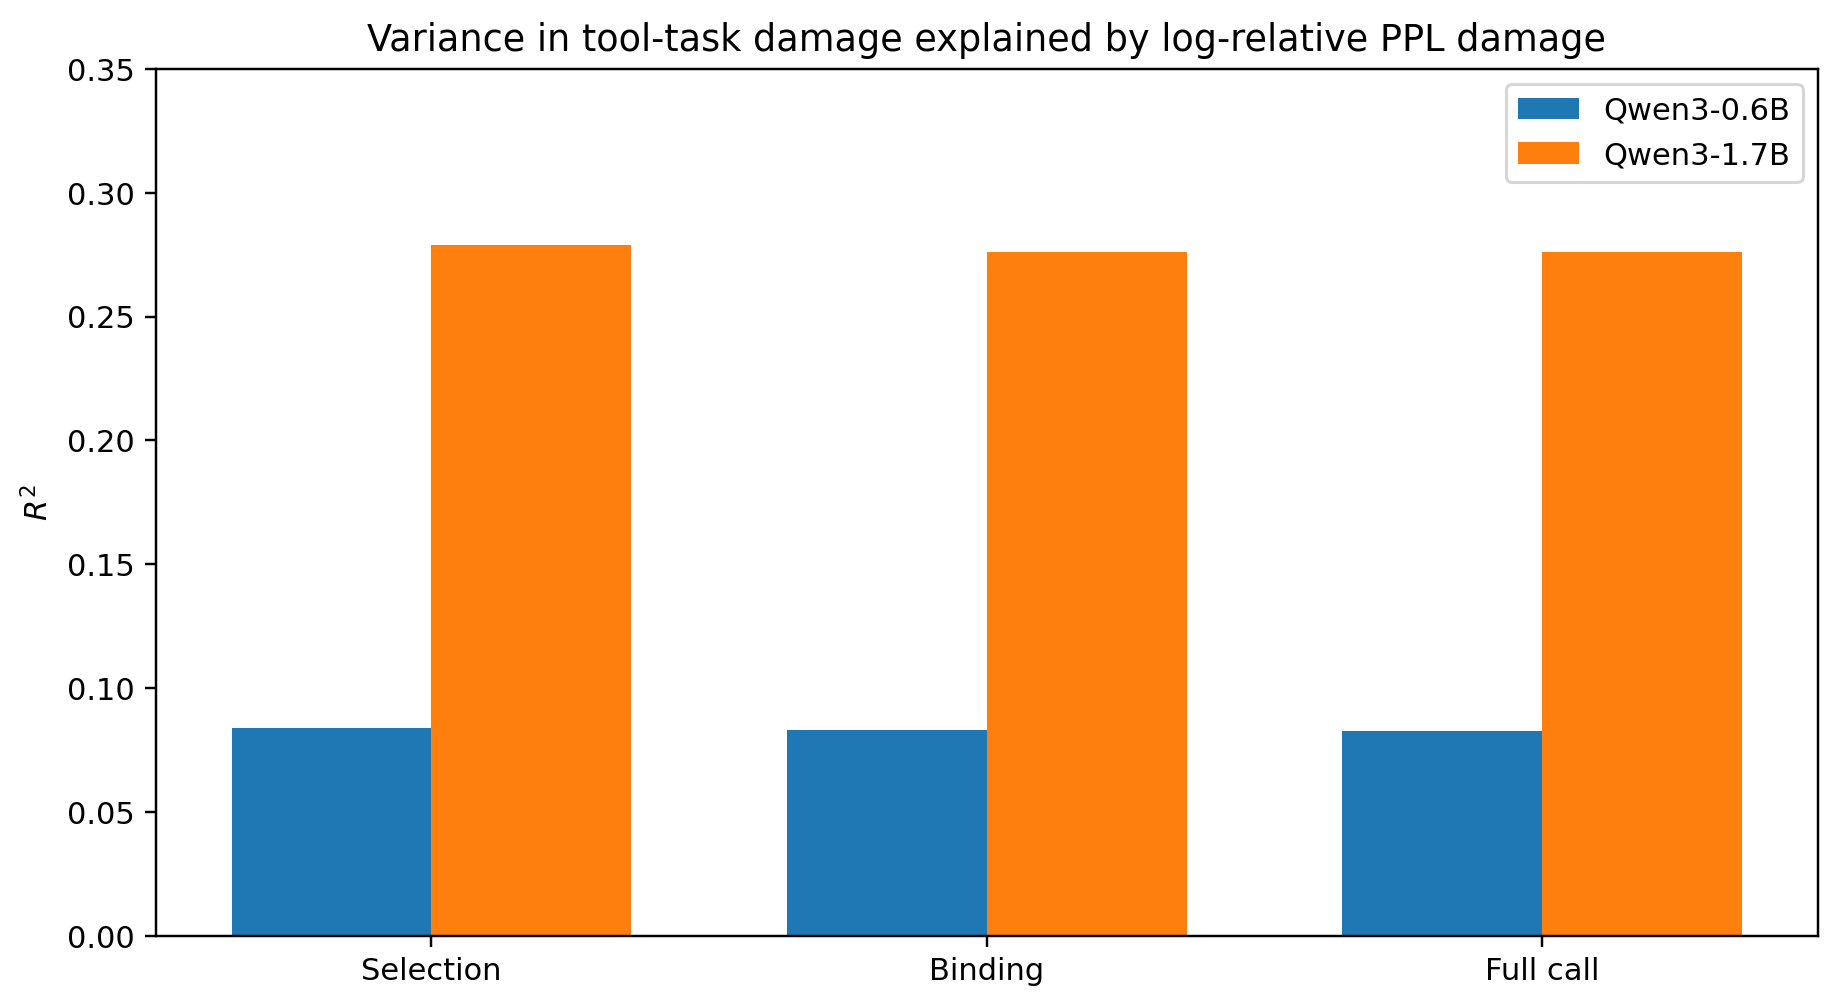
\includegraphics[width=\columnwidth]{figure4_r2.png}
\caption{Variance in target damage explained by the primary log-relative perplexity model.}
\label{fig:r2}
\end{figure}

\subsection{Conservative excess-sensitive blocks}
For Qwen3-0.6B, eight zero-based block indices survive the conservative checks across all three target metrics:
\begin{equation}
\{6,9,10,14,18,19,21,26\}.
\end{equation}
Each reduces tool selection from 16/20 intact to 0/20 on the observed discovery examples. Layer 14 is illustrative: mean perplexity increases by only 0.78\%, while selection falls by 80 percentage points. Its selection residual is 33.3 points with an approximate simultaneous band of 26.0--40.6 points.

For Qwen3-1.7B, the conservative set is
\begin{equation}
\{11,24,27\}.
\end{equation}
The intact model scores 20/20 selection and 19/20 binding/full-call. Table~\ref{tab:17} shows the strongest 1.7B results.

\begin{table}[t]
\centering
\caption{Qwen3-1.7B conservative excess-sensitive blocks. ``Residual'' is selection damage beyond the primary fitted perplexity relation.}
\label{tab:17}
\begin{tabular}{rrrr}
\toprule
Layer & PPL $\Delta$ & Sel. damage & Residual \\
\midrule
11 & +29.8\% & 100 pp & 78.5 pp \\
24 & +41.1\% & 95 pp & 73.0 pp \\
27 & +23.7\% & 85 pp & 63.9 pp \\
\bottomrule
\end{tabular}
\end{table}

Layer 2 demonstrates why regression residuals cannot be interpreted mechanically: it has a large linear-model excess but roughly 691$\times$ perplexity ratio and a zero isotonic residual, placing it in a catastrophic general-damage regime.

\begin{figure*}[t]
\centering
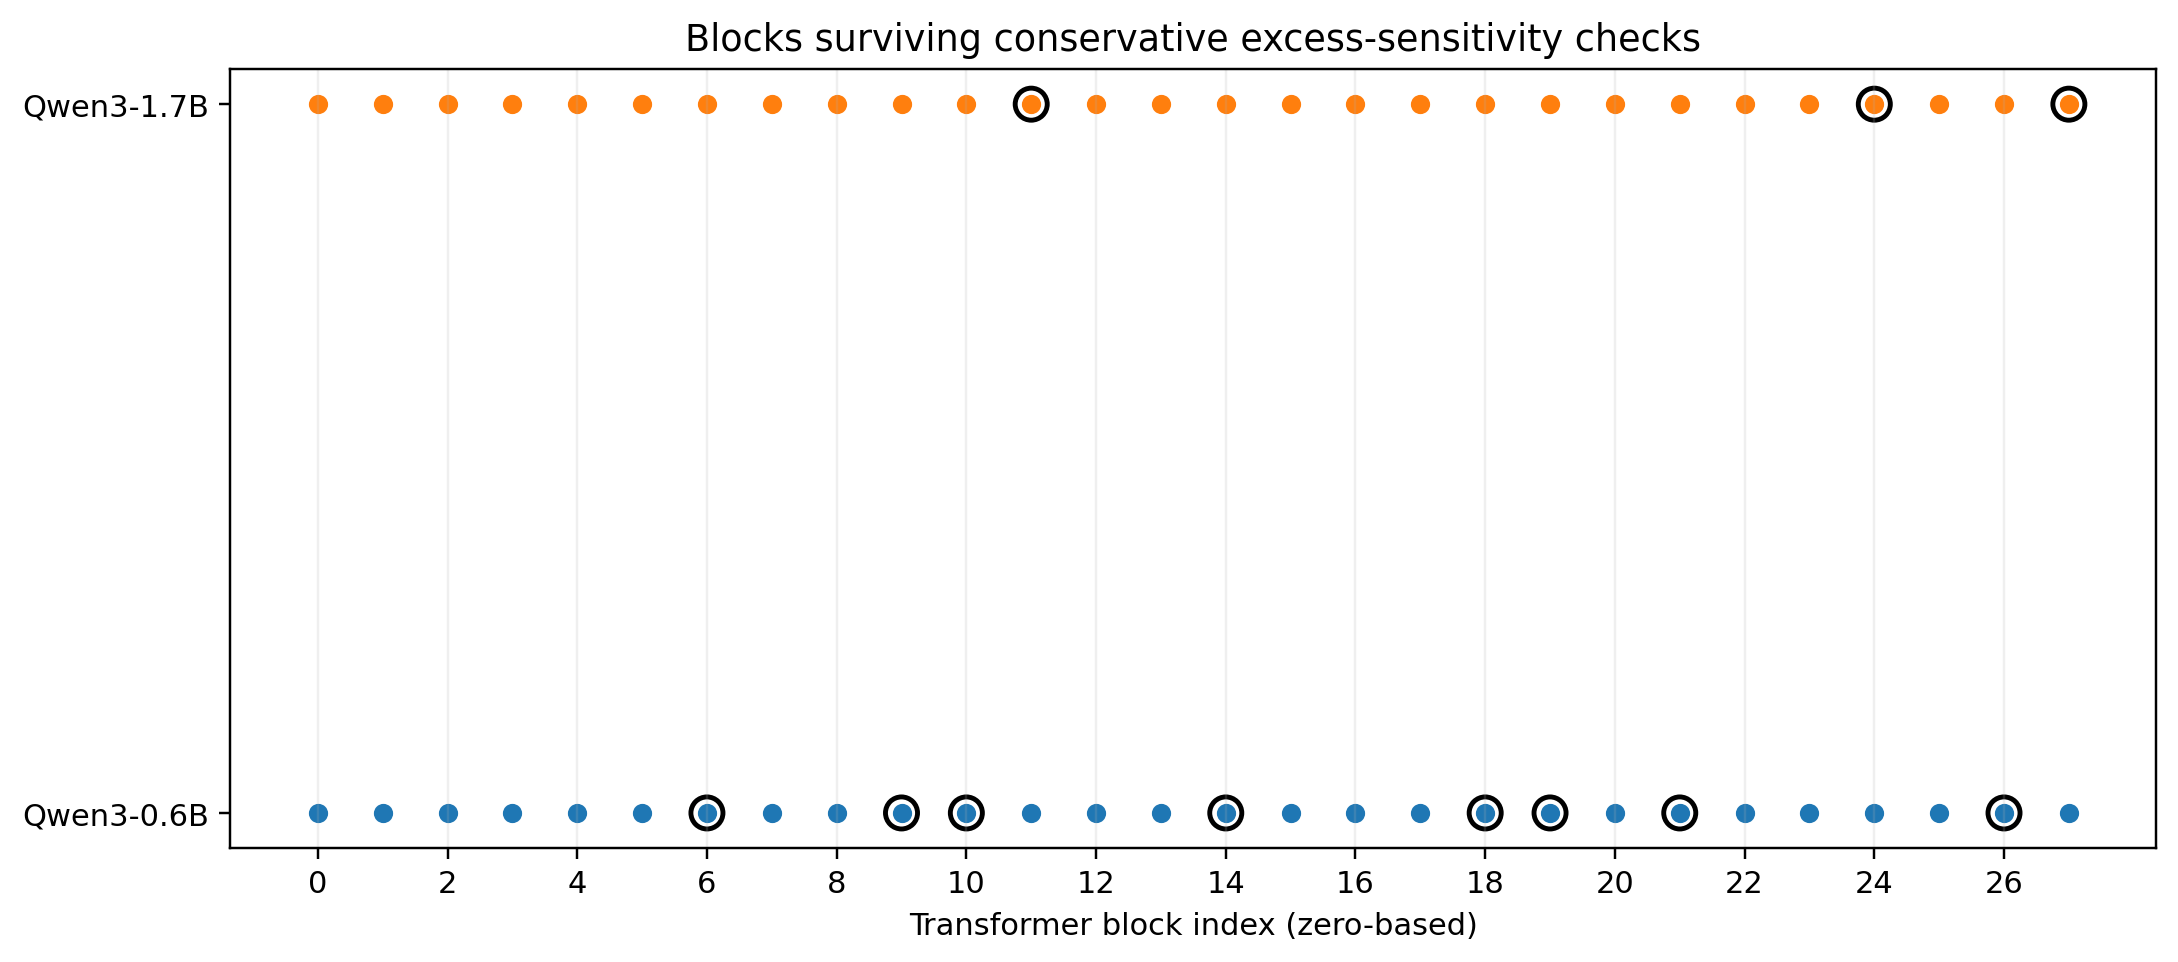
\includegraphics[width=0.86\textwidth]{figure3_robust_layers.png}
\caption{Blocks surviving conservative excess-sensitivity checks. The absence of overlap across identical indices is descriptive; it does not prove that a capability ``moves'' with scale.}
\label{fig:layers}
\end{figure*}

\subsection{Weak cross-size agreement}
The conservative sets do not overlap. Aligned-index residual-profile Spearman correlations are 0.277 for selection, 0.272 for binding, and 0.290 for full-call correctness. These weak associations contrast with substantially stronger previously measured raw perplexity-sensitivity alignment across the same two sizes.

\begin{figure}[t]
\centering
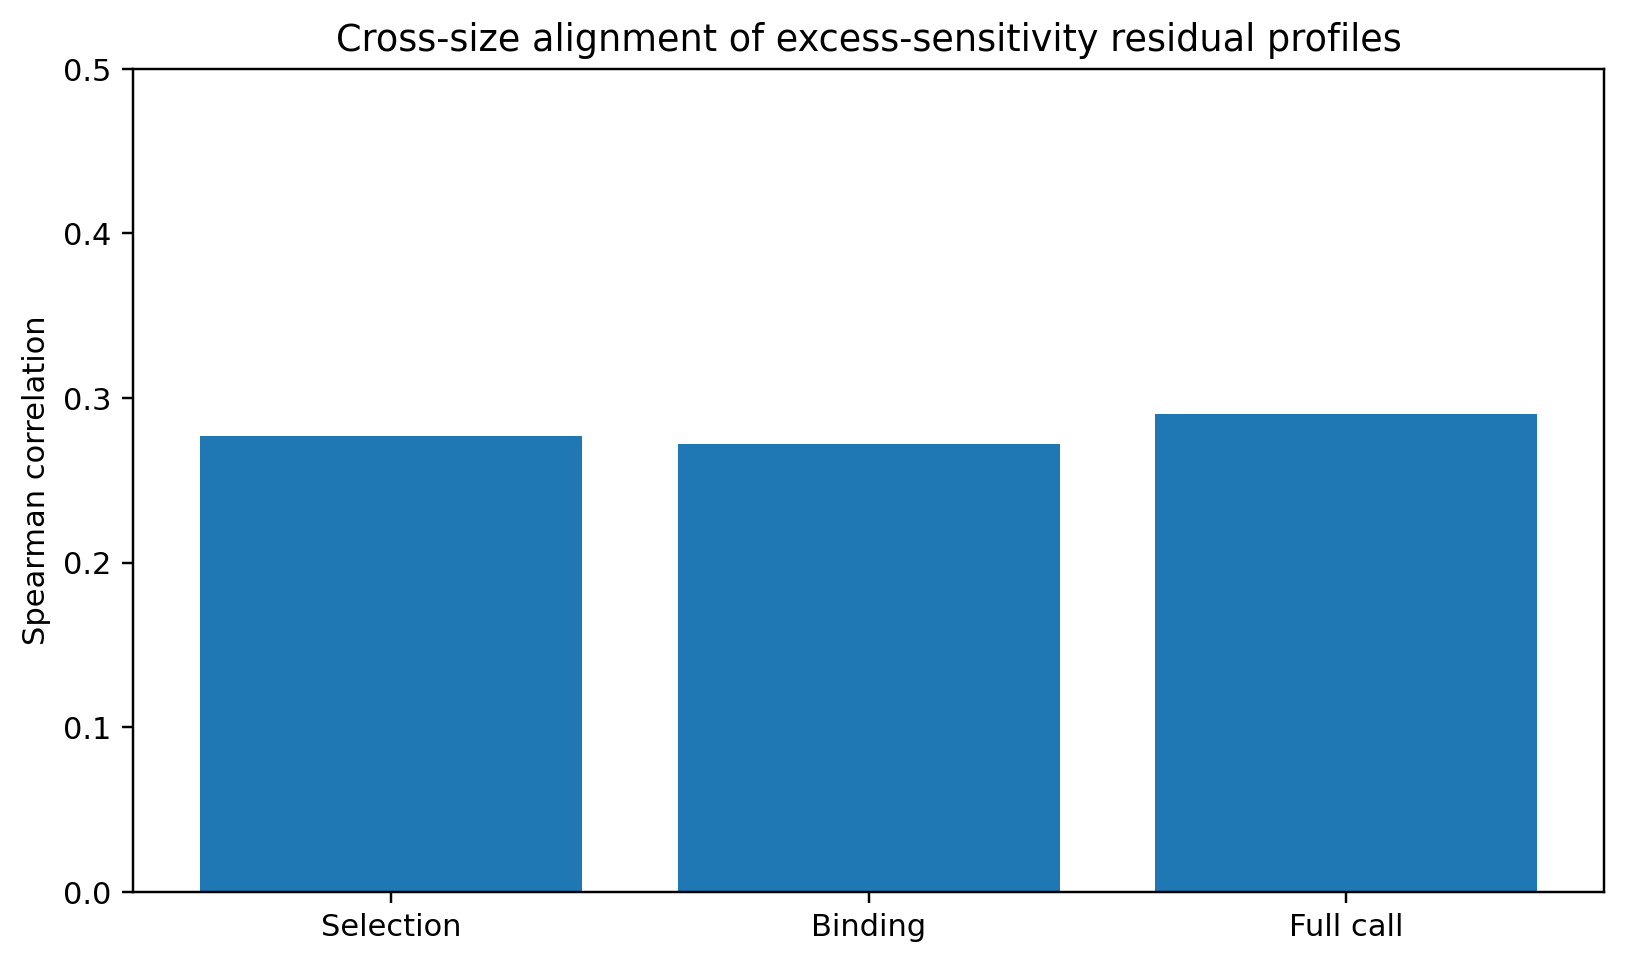
\includegraphics[width=\columnwidth]{figure5_cross_size_corr.png}
\caption{Cross-size Spearman correlations of residual tool-sensitivity profiles.}
\label{fig:corr}
\end{figure}

The result should not be read as evidence that a fixed capability changes physical location with parameter count. Ceiling effects, sample composition, model quality, regression misspecification, redundancy, and proxy limitations remain alternative explanations.

\section{Discussion}
The scope limits should be kept in view when interpreting every result: the primary endpoint uses only 20 discovery tool examples, the collateral proxy is perplexity on five documents, both models are from the Qwen family, the specificity analysis is post hoc, and Phase 5 contains no held-out per-layer intervention map. These constraints make the study appropriate as a measurement result rather than a general localization claim.

\subsection{Sensitivity is not localization}
A reproducible intervention effect establishes that bypassing a component predictably changes behavior under the tested setup. It does not prove that the component uniquely stores or implements an abstract capability. The component may be a source, router, integrator, or one of several redundant paths. Figure~\ref{fig:claim} summarizes this evidence ladder.

This distinction is consistent with the localization/editing mismatch \cite{hase2023localization} and evidence for distributed, functionally equivalent computation paths \cite{hochman2026factual}.

\subsection{General importance versus target sensitivity}
Raw target damage confounds general fragility with task-specific dependence. Conditioning on perplexity changes the interpretation: blocks 11, 24, and 27 in 1.7B and a broader set in 0.6B cause tool-task failures larger than the fitted general-damage proxy predicts. This is stronger evidence than raw ranking alone, but remains conditional on an imperfect proxy. In particular, we cannot rule out that replacing the five-document perplexity proxy with a broader collateral-behavior panel would materially change the excess-sensitive sets.

A stronger future design should replace the single perplexity proxy with a panel of unrelated behavioral controls and directly test a contrast such as
\begin{equation}
\mathrm{Specificity}_{l,c}=D_{l,c}-\mathbb{E}[D_{l,\mathrm{collateral}}].
\end{equation}

\subsection{Implications for capability engineering}
The practical value of localization is predictive utility: does a localization score tell us where to edit, prune, or adapt? The present experiment does not answer this. The natural follow-up is equal-budget adaptation at high-ranked, low-ranked, and random locations. If anatomy predicts selective adaptation, it becomes an engineering tool. If not, the result would extend known localization/editability mismatches from factual editing to behavioral capabilities.

\section{Limitations}
The study has important limitations. (1) Both primary models belong to one model family, so the empirical findings should not be generalized to all LLM architectures. (2) Only whole-block interventions are analyzed; MLP-, attention-, head-, and feature-level interventions may yield different maps. (3) The primary tool endpoint contains only 20 distinct discovery examples; this is the largest limitation on behavioral generalization and makes the present result exploratory rather than population-level. (4) Perplexity is computed from five documents and cannot establish preservation of unrelated capabilities; a richer collateral task panel could change the fitted general-damage relation and the resulting excess-sensitive sets. (5) Phase 5 contains no held-out per-layer validation map. (6) The specificity analysis is post hoc with respect to already observed model outputs. (7) Qwen3-1.7B starts at or near ceiling, while some interventions saturate at zero. (8) Binding and full-call are highly collinear. (9) historical abstention, reasoning, and formatting measurements have audited limitations and are excluded from headline claims. (10) Behavioral damage does not identify where information is represented, nor does it establish editability.

\section{Conclusion}
Whole-block interventions in the two studied Qwen models reveal reproducible differences in tool-calling sensitivity across depth. Some blocks cause tool-task degradation substantially larger than predicted by their retained perplexity degradation, but conservative excess-sensitivity patterns differ strongly across Qwen3-0.6B and 1.7B. The evidence therefore supports a narrow conclusion: \textbf{layerwise causal interventions can identify reproducible regions of behavioral sensitivity, but additional evidence is required before such sensitivity is interpreted as a stable capability location.} The most informative next evidence would be cross-family replication, a truly held-out per-layer intervention map, finer-grained MLP/attention interventions, and equal-budget editing or adaptation experiments that test whether sensitivity rankings predict where behavior can be changed selectively.

\section*{Reproducibility Statement}
The analysis is derived from preserved Phase 5 evidence and introduces no new inference. The complete Qwen3-1.7B bundle contains 101 verified files (9,203,408 source bytes). Its preserved archive SHA-256 is \texttt{2a67da263a35f34989311ca0620a5301}\-\texttt{ee1f9f98000f18a0911e460d22a6ed45}; the per-file manifest SHA-256 is \texttt{3f7f4f0334b8b5dc89a6fdb8c8825f3}\-\texttt{63278ec994dcb8967daa884030cef36e7}. The preservation and specificity analysis are recorded on repository commit \texttt{9c90e4c}. Analysis code, CSV outputs, bootstrap artifacts, verification records, and rendered figures are versioned with the evidence report.

\appendix
\section{Interpretation Guide}
We recommend the following terminology for future work:
\begin{itemize}
\item \textbf{Layer sensitivity}: behavioral damage under a specified layer intervention.
\item \textbf{Excess sensitivity}: target damage larger than predicted by an explicitly stated collateral/general-damage model.
\item \textbf{Capability-specific localization}: a stronger claim requiring appropriate collateral controls, replication, and intervention robustness.
\item \textbf{Stable capability location}: an even stronger claim requiring stability across samples, methods, model instances, and ideally families.
\end{itemize}

\begin{thebibliography}{9}
\bibitem{zhao2024layer} Zheng Zhao, Yftah Ziser, and Shay B. Cohen. Layer by Layer: Uncovering Where Multi-Task Learning Happens in Instruction-Tuned Large Language Models. EMNLP, 2024. doi:10.18653/v1/2024.emnlp-main.847.
\bibitem{alkhamissi2025llm} Badr AlKhamissi, Greta Tuckute, Antoine Bosselut, and Martin Schrimpf. The LLM Language Network: A Neuroscientific Approach for Identifying Causally Task-Relevant Units. NAACL-HLT, 2025. doi:10.18653/v1/2025.naacl-long.544.
\bibitem{hase2023localization} Peter Hase, Mohit Bansal, Been Kim, and Asma Ghandeharioun. Does Localization Inform Editing? Surprising Differences in Causality-Based Localization vs. Knowledge Editing in Language Models. NeurIPS, 2023.
\bibitem{zhang2024patching} Fred Zhang and Neel Nanda. Towards Best Practices of Activation Patching in Language Models: Metrics and Methods. ICLR, 2024.
\bibitem{hochman2026factual} Hail Hochman, Natalie Shapira, and Yoav Goldberg. Factual Retrieval in LLMs Is a Redundant, Distributed and Non-Contiguous Process. ACL, 2026. doi:10.18653/v1/2026.acl-long.2168.
\bibitem{wang2022skill} Xiaozhi Wang, Kaiyue Wen, Zhengyan Zhang, Lei Hou, Zhiyuan Liu, and Juanzi Li. Finding Skill Neurons in Pre-trained Transformer-based Language Models. EMNLP, 2022. doi:10.18653/v1/2022.emnlp-main.765.
\bibitem{dai2022knowledge} Damai Dai, Li Dong, Yaru Hao, Zhifang Sui, Baobao Chang, and Furu Wei. Knowledge Neurons in Pretrained Transformers. ACL, 2022. doi:10.18653/v1/2022.acl-long.581.
\bibitem{meng2022rome} Kevin Meng, David Bau, Alex Andonian, and Yonatan Belinkov. Locating and Editing Factual Associations in GPT. NeurIPS, 2022.
\bibitem{yan2025robust} Jianhao Yan, Futing Wang, Yun Luo, Yafu Li, and Yue Zhang. Keys to Robust Edits: From Theoretical Insights to Practical Advances. ACL, 2025. doi:10.18653/v1/2025.acl-long.1099.
\bibitem{das2025toxic} Anubrata Das, Manoj Kumar, Ninareh Mehrabi, Anil Ramakrishna, Anna Rumshisky, Kai-Wei Chang, Aram Galstyan, Morteza Ziyadi, and Rahul Gupta. On Localizing and Deleting Toxic Memories in Large Language Models. Findings of NAACL, 2025. doi:10.18653/v1/2025.findings-naacl.129.
\bibitem{hu2025trimllm} Lanxiang Hu, Tajana Rosing, and Hao Zhang. TrimLLM: Progressive Layer Dropping for Domain-Specific LLMs. ACL, 2025. doi:10.18653/v1/2025.acl-long.33.
\end{thebibliography}
\end{document}
